\documentclass[]{beamer}
\mode<presentation>
{
\usetheme{-bjeldbak/beamerthemebjeldbak}
  \usecolortheme{default} % or try albatross, beaver, crane, ...
  \usefonttheme{default}  % or try serif, structurebold, ...
\usepackage[english]{babel}
\usepackage[utf8x]{inputenc}
 \usepackage{subfiles}
 \usepackage{bm}
\usepackage{graphicx}
 \usepackage{relsize}
\setbeamertemplate{caption}{\insertcaption}
  \setbeamertemplate{navigation symbols}{}
  \setbeamertemplate{caption}[numbered]
\setbeamertemplate{navigation symbols}[horizontal]
} 

\begin{document}
 \graphicspath{{images/}}

\title{Innappropriate parameterization of fossilized birth-death models causes incorrect estimates of node ages}
\author{April M. Wright \dag \ddag \\ Tracy A. Heath \dag}
\institute{\dag Iowa State University,  \ddag University of Kansas}
\date{6.19.2016}
\maketitle

\begin{frame}
\frametitle{Fossilized Birth-Death Process}
\end{frame}

\begin{frame}
\frametitle{Fossilized Birth-Death Process}
\begin{itemize}
\item A probabilistic model for estimating divergence times
\end{itemize}
\end{frame}

\begin{frame}
\frametitle{Fossilized Birth-Death Process}
\begin{itemize}
\item A probabilistic model for estimating divergence times
\item Treat fossil and molecular occurrence times as part of the same process
\end{itemize}
\end{frame}

\begin{frame}
\frametitle{Fossilized Birth-Death Process}
\begin{itemize}
\item A probabilistic model for estimating divergence times
\item Treat fossil and molecular occurrence as part of the same process 
\begin{itemize}
	\item Avoid calibration densities 
\end{itemize}	
\end{itemize}
\end{frame}

\begin{frame}
\frametitle{Fossilized Birth-Death Process}
\begin{itemize}
\item A probabilistic model for estimating divergence times
\item Treat fossil and molecular occurrence as part of the same process 
\begin{itemize}
	\item Avoid calibration densities 
	\item Use multiple fossils per node
\end{itemize}	
\end{itemize}
\end{frame}

\begin{frame}
\frametitle{Fossilized Birth-Death Process}
\begin{columns}
\begin{column}{0.5\textwidth}
\includegraphics[scale=.25]{images/CleanCopy_graphical} \\
\end{column}
\begin{column}{0.4\textwidth}
\begin{tabular}{ l  | r }
Parameter & Meaning \\
\hline 
\end{tabular}
\end{column}
\end{columns}
\end{frame}

\begin{frame}
\frametitle{Fossilized Birth-Death Process}
\begin{columns}
\begin{column}{0.5\textwidth}
\includegraphics[scale=.25]{images/Lambdahighlight} \\
\end{column}
\begin{column}{0.4\textwidth}
\begin{tabular}{ l  | r }
Parameter & Meaning \\
\hline 
\lambda & Speciation Rate
\end{tabular}
\end{column}
\end{columns}
\end{frame}


\begin{frame}
\frametitle{Fossilized Birth-Death Process}
\begin{columns}
\begin{column}{0.5\textwidth}
\includegraphics[scale=.25]{images/muhighlight} \\
\end{column}
\begin{column}{0.4\textwidth}
\begin{tabular}{ l  | r }
Parameter & Meaning \\
\hline 
\lambda & Speciation Rate \\
\mu & Extinction Rate \\ 
\end{tabular}
\end{column}
\end{columns}
\end{frame}

\begin{frame}
\frametitle{Fossilized Birth-Death Process}
\begin{columns}
\begin{column}{0.5\textwidth}
\includegraphics[scale=.25]{images/psilight} \\
\end{column}
\begin{column}{0.4\textwidth}
\begin{tabular}{ l  | r }
Parameter & Meaning \\
\hline 
\lambda & Speciation Rate \\
\mu & Extinction Rate \\ 
\psi & Paleo Sampling\\
\end{tabular}
\end{column}
\end{columns}

\end{frame}

\begin{frame}
\frametitle{Fossilized Birth-Death Process}
\begin{columns}
\begin{column}{0.5\textwidth}
\includegraphics[scale=.25]{images/rhohighlight} \\
\end{column}
\begin{column}{0.4\textwidth}
\begin{tabular}{ l  | r }
Parameter & Meaning \\
\hline 
\lambda & Speciation Rate \\
\mu & Extinction Rate \\ 
\psi & Paleo Sampling\\
\rho & Extant Sampling \\
\end{tabular}
\end{column}
\end{columns}
\end{frame}

\begin{frame}
\frametitle{Fossilized Birth-Death Process}
\begin{columns}
\begin{column}{0.5\textwidth}
\includegraphics[scale=.25]{images/turnhighlight} \\
\end{column}
\begin{column}{0.5\textwidth}
\[Turnover = \mu/\lambda \]
\end{column}
\end{columns}
\end{frame}

\begin{frame}
\frametitle{Fossilized Birth-Death Process}
\begin{itemize}
\item A probabilistic model for estimating divergence times
\item Treat fossil and molecular data as part of the same process 
\begin{itemize}
	\item Avoid calibration densities 
	\item Use multiple fossils per node
\end{itemize}
\item Account for presence of lineages which have sampled descendants	
\end{itemize}
\end{frame}

\begin{frame}
\frametitle{Fossilized Birth-Death Process}
\begin{itemize}
\item A probabilistic model for estimating divergence times
\item Treat fossil and molecular data as part of the same process 
\begin{itemize}
	\item Avoid calibration densities 
	\item Use multiple fossils per node
\end{itemize}
\item \textbf{Account for presence of lineages which have sampled descendants}	
\end{itemize}
\end{frame}

\begin{frame}
\frametitle{Sampled ancestor models}
\begin{figure}
\includegraphics[scale=.25]{images/SA} \\
Image: Stadler 2010, Journal of Theoretical Biology
\end{figure}
\end{frame}



\begin{frame}
\frametitle{Divergence Dating and Reasonable Ages}
\end{frame}

\begin{frame}
\frametitle{Divergence Dating and Reasonable Ages}
\begin{itemize}
\item Empirical studies have noted that dated trees made using combined molecular+morphological data tend to produce older ages than studies with molecular data and node calibrations
\end{itemize}
\end{frame}

\begin{frame}
\frametitle{Divergence Dating and Reasonable Ages}
\begin{itemize}
\item Empirical studies have noted that dated trees made using combined molecular+morphological data tend to produce older ages than studies with molecular data and node calibrations
\end{itemize}
\end{frame}

\begin{frame}
\frametitle{Our Research Question}
Is this an inherent property of 'total-evidence' approaches, or is this related to model misspecification?
\end{frame}

\begin{frame}
\frametitle{Our Research Question}
\begin{figure}
\includegraphics[scale=.25]{images/SA} \\
Image: Stadler 2010, Journal of Theoretical Biology
\end{figure}
\end{frame}

\begin{frame}
\frametitle{Our Research Question}
\begin{figure}
\includegraphics[scale=.25]{images/OneBranch} \\
No Sampled Ancestors Model
\end{figure}
\end{frame}


\begin{frame}
\frametitle{Our Research Question}
\begin{columns}
\begin{column}{0.5\textwidth}
\includegraphics[scale=.25]{images/OneBranchSolo} \\
\end{column}
\begin{column}{0.5\textwidth}
\begin{center}
No Sampled \\ Ancestors Model \\
\[ \mathlarger{\boldsymbol{\lambda}} \\
\rho \\
\mu \\
 \psi \]
\end{center}
\end{column}
\end{columns}
\end{frame}

\begin{frame}
\frametitle{Our Research Question}
\includegraphics[scale=.25]{images/5sa} \\
\end{frame}

\begin{frame}
\frametitle{Our Research Question}
\begin{columns}
\begin{column}{0.5\textwidth}
\includegraphics[scale=.25]{images/FiveBranch} \\
\end{column}
\begin{column}{0.5\textwidth}
\begin{center}
Sampled \\ Ancestors Model \\
\[\lambda \\
\rho \\
\mu \\
 \psi \]
\end{center}
\end{column}
\end{columns}
\end{frame}

\begin{frame}
\frametitle{Our Research Question}
\begin{columns}
\begin{column}{0.5\textwidth}
\includegraphics[scale=.25]{images/FiveBranch} \\
\end{column}
\begin{column}{0.5\textwidth}
\begin{center}
Sampled \\ Ancestors Model \\
\[\mathlarger{\mathlarger{\mathlarger{\boldsymbol{\lambda}}}}\\
\rho \\
\mu \\
 \psi \]
\end{center}
\end{column}
\end{columns}
\end{frame}

\begin{frame}
\frametitle{Turnover}
\includegraphics[scale=.4]{images/prob_ancs} \\

\end{frame}

\begin{frame}
\frametitle{Methods}
\end{frame}

\begin{frame}
\frametitle{Methods}
\begin{itemize}
\item Simulations
\end{itemize}
\end{frame}

\begin{frame}
\frametitle{Methods}
\begin{itemize}
\item Simulations
\begin{itemize}
\item 25 extant tips with nucleotide sequence data
\item Variable number of fossil tips, without data
\end{itemize}
\end{itemize}
\end{frame}

\begin{frame}
\frametitle{Methods}
\begin{itemize}
\item Simulations
\begin{itemize}
\item 25 extant tips with nucleotide sequence data
\item Variable number of fossil tips, without data
\item Simulate different trees and fossils with values for \lambda, \mu ,  \psi
\end{itemize}
\end{itemize}
\end{frame}

\begin{frame}
\frametitle{Methods}
\begin{itemize}
\item Simulations
\begin{itemize}
\item 25 extant tips with nucleotide sequence data
\item Variable number of fossil tips, without data
\item Simulate different trees and fossils with values for \lambda, \mu ,  \psi
\end{itemize}
\item Strict molecular clock for sequence data
\end{itemize}
\end{frame}

\begin{frame}
\frametitle{Methods}
\begin{itemize}
\item Empirical Data
\begin{itemize}
\item Bear data set of Krause, 2008; Abella, 2012.
\end{itemize}
\end{itemize}
\end{frame}

\begin{frame}
\frametitle{Methods}
\begin{itemize}
\item Estimation
\begin{itemize}
\item Estimate a tree for each dataset using both sampled ancestor and non-sampled ancestor models in BEAST2
\end{itemize}
\end{itemize}
\end{frame}

\begin{frame}
\begin{center}
\begin{figure}
\frametitle{Results -  Simulations}
Low turnover, low sampling  \\
20\% of fossils are sampled ancestors \\
\boldsymbol{\lambda} \mu \psi   \rho \\
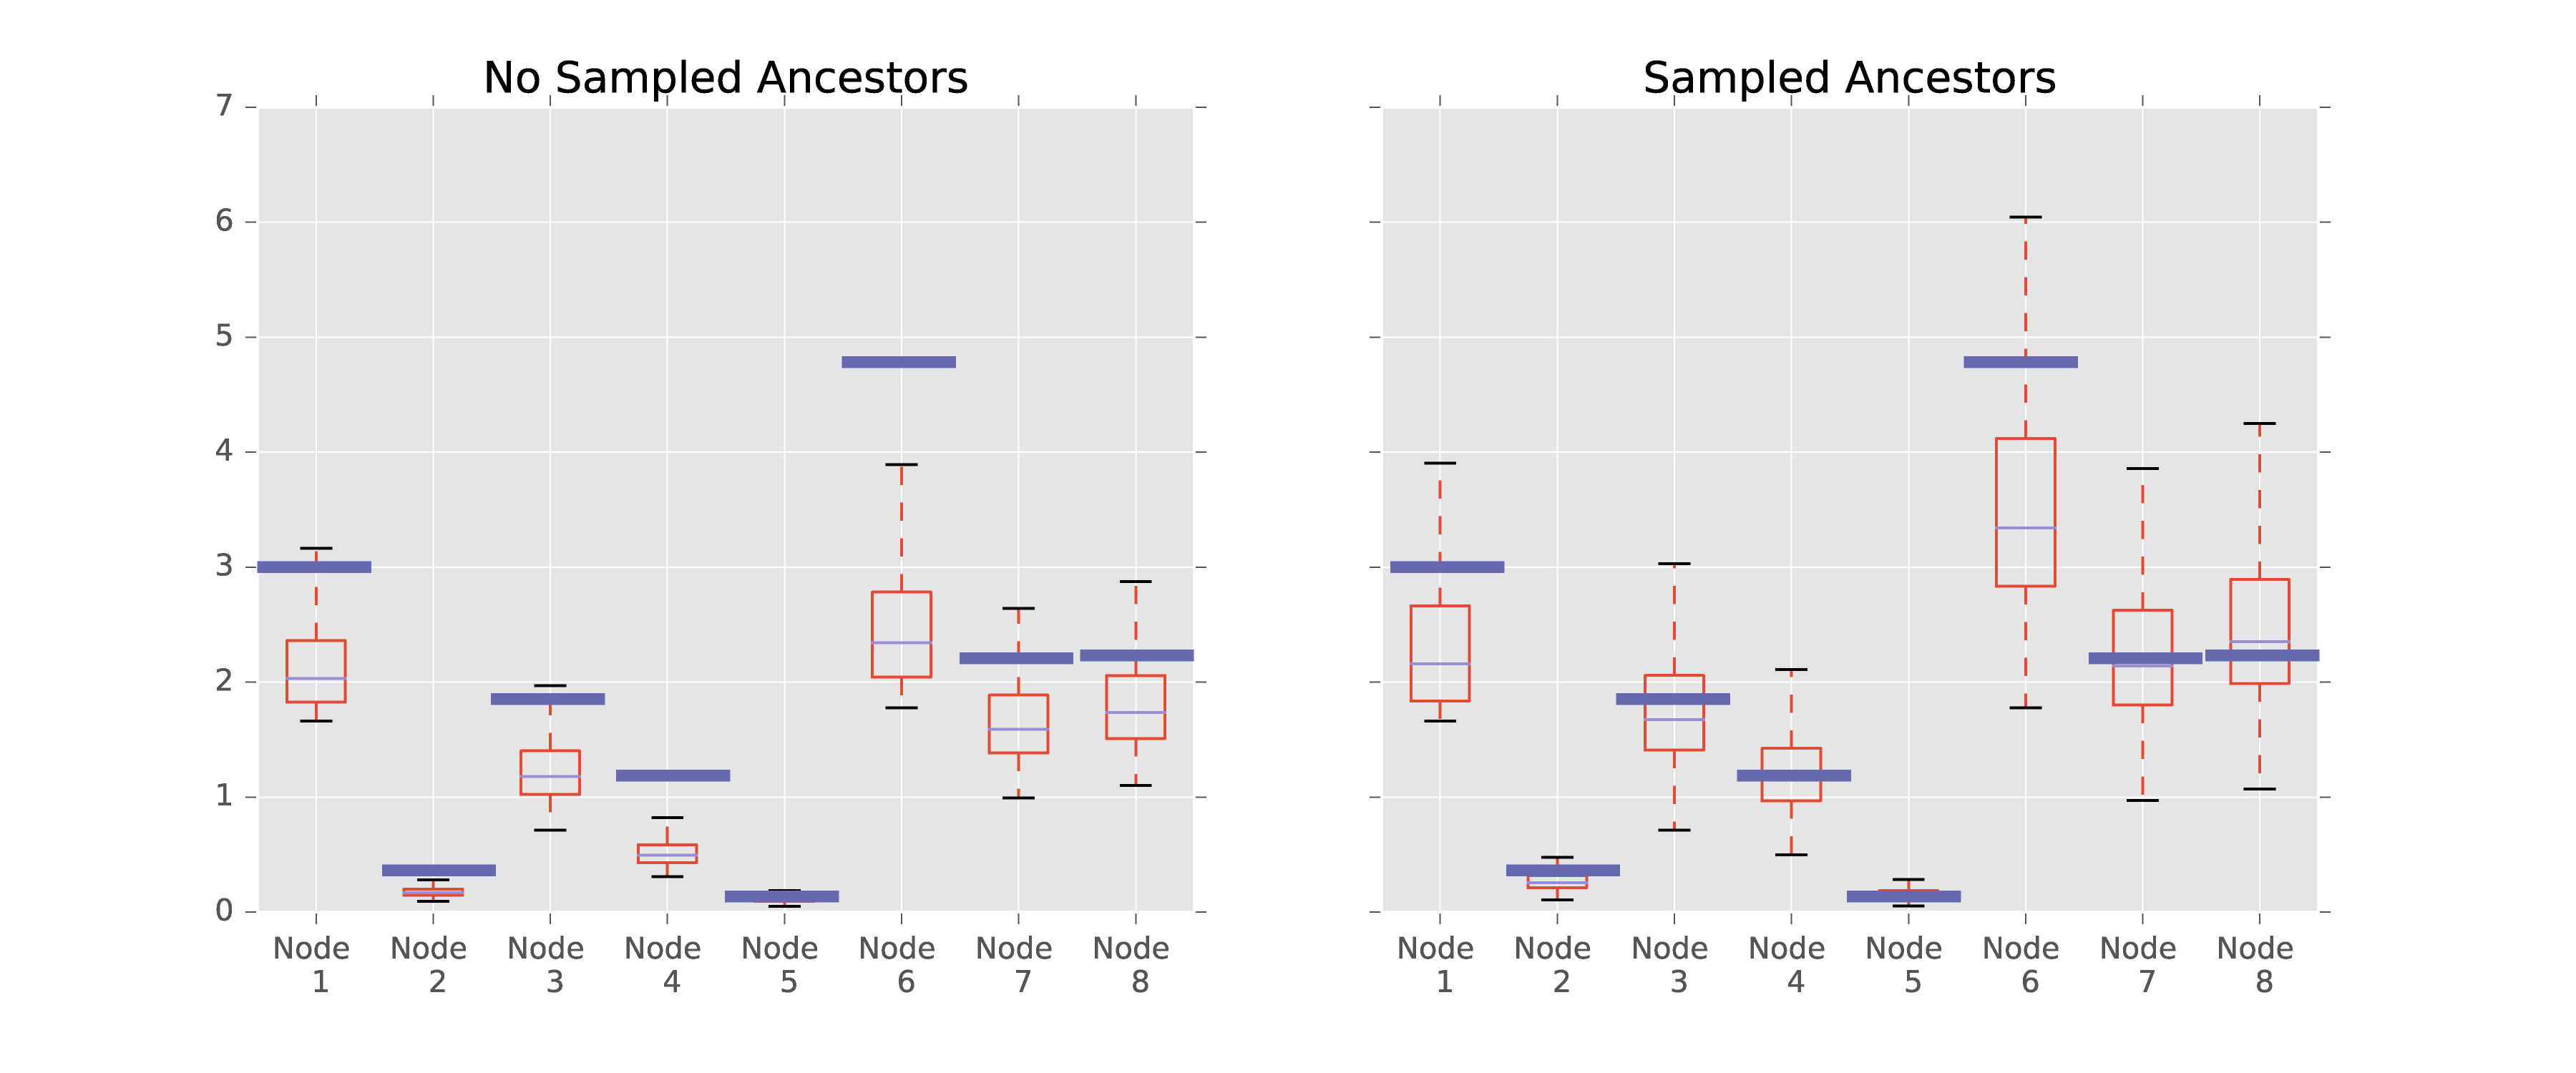
\includegraphics[scale=0.4]{images/LowTurnLowSampnodes}
\end{figure}
\end{center}
\end{frame}

\begin{frame}
\begin{center}
\begin{figure}
\frametitle{Results -  Simulations}
Low turnover, low sampling  \\
20\% of fossils are sampled ancestors \\
\boldsymbol{\lambda} \mu \psi   \rho \\
\includegraphics[scale=0.4]{images/LowTurnLowSamp}
\end{figure}
\end{center}
\end{frame}


\begin{frame}
\frametitle{Results -  Simulations}
\begin{center}
\begin{figure}
High turnover, low sampling  \\
62\% of fossils are sampled ancestors \\
\mathlarger{\mathlarger{\lambda}} \mu   \psi   \rho \\
Rerunning.
\end{figure}
\end{center}
\end{frame}

\begin{frame}
\frametitle{Results -  Simulations}
\begin{center}
\begin{figure}
Low turnover, high sampling  \\
77\% of fossils are sampled ancestors \\
\boldsymbol{\lambda} \mu  \psi   \rho \\
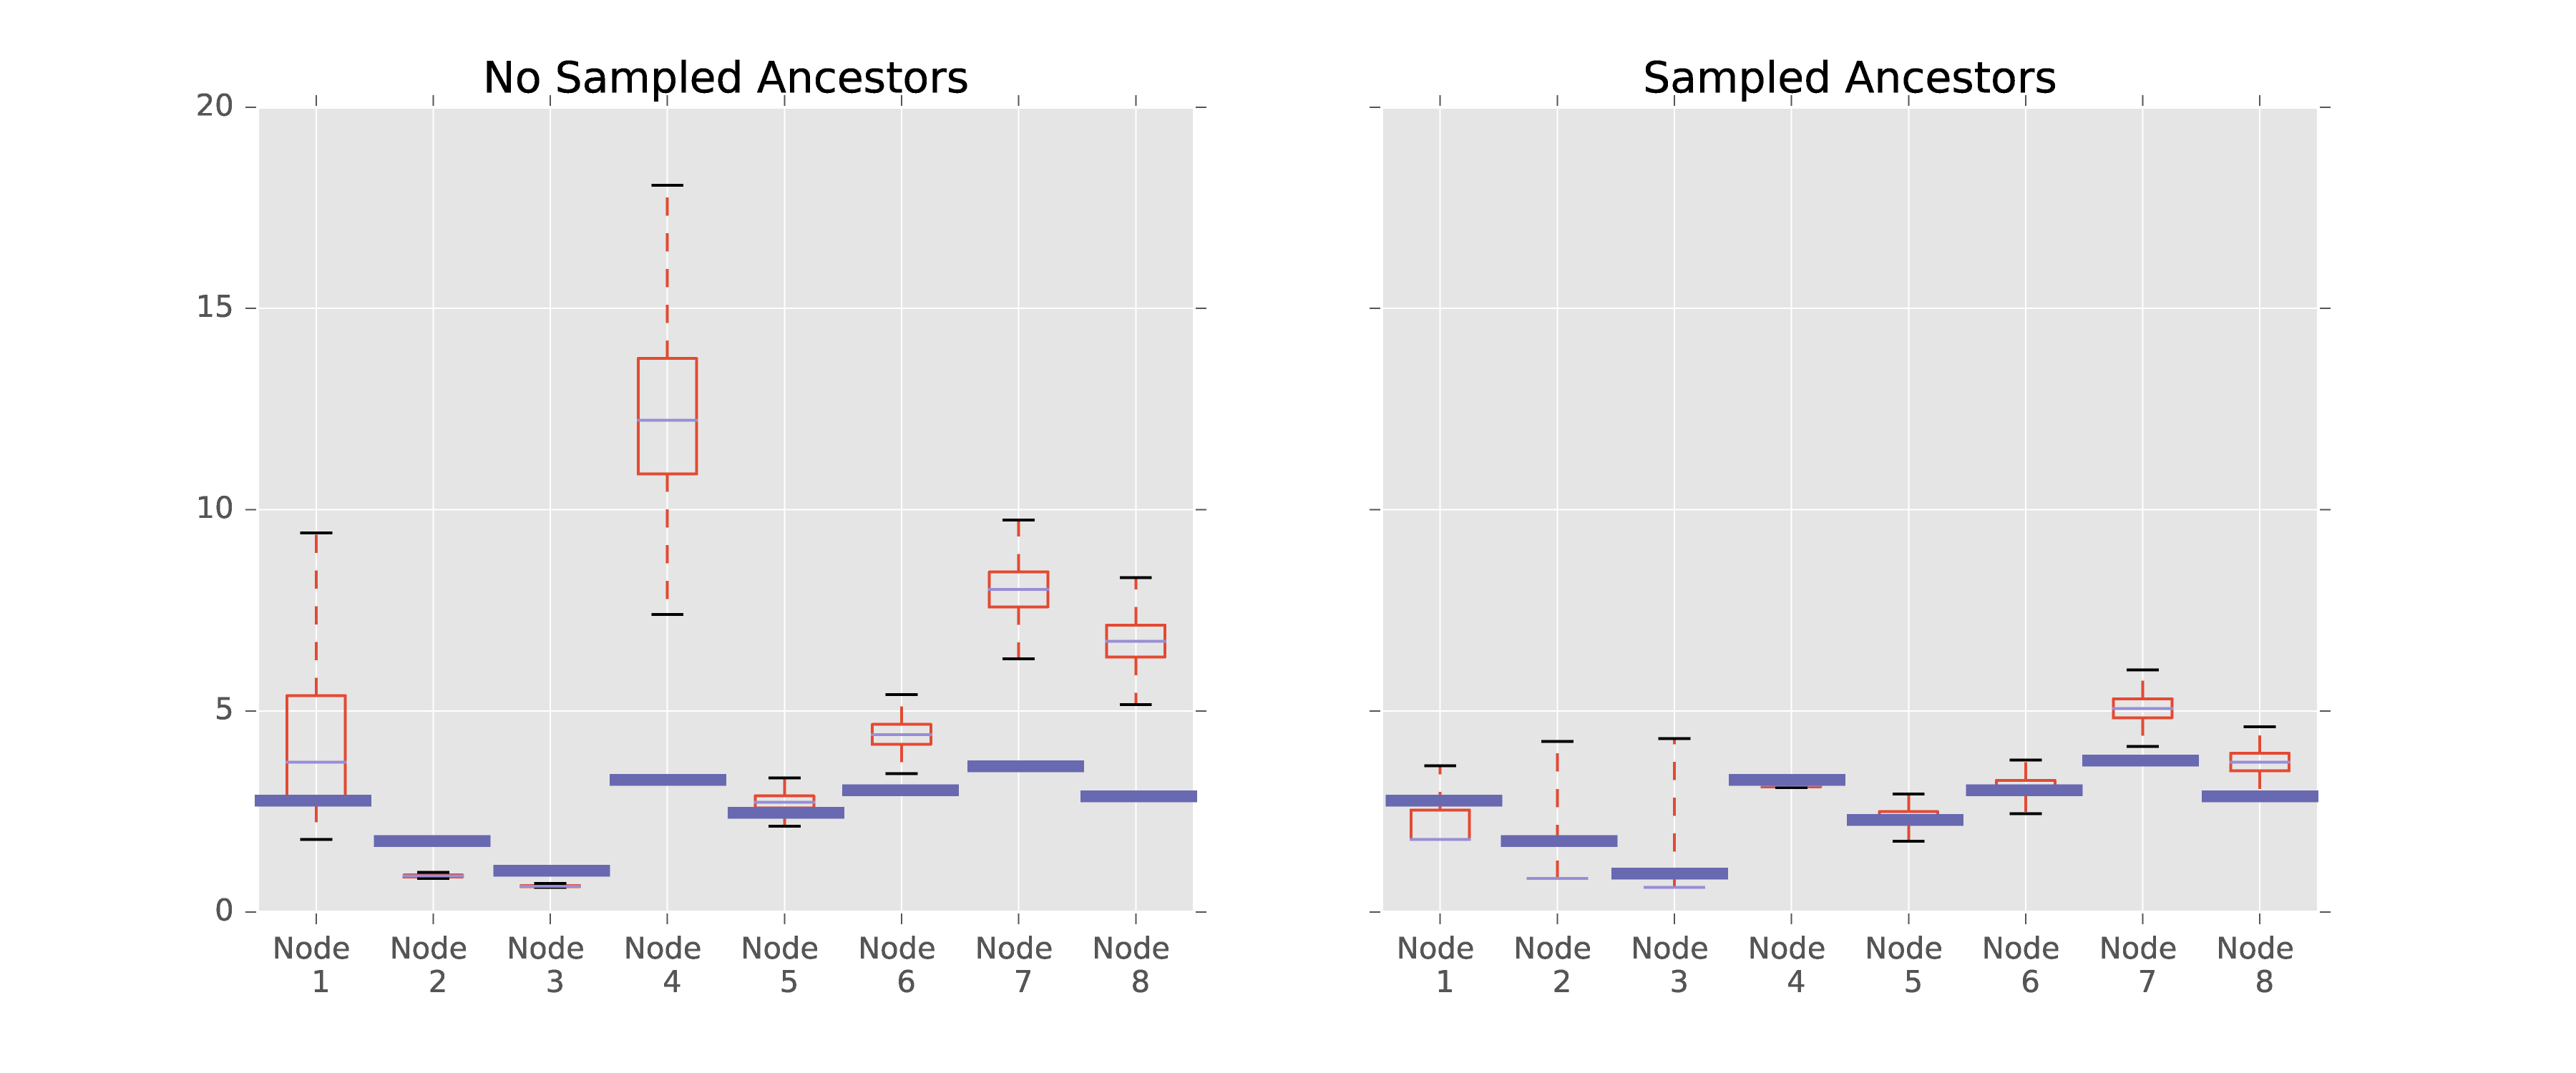
\includegraphics[scale=0.4]{images/LowTurnHighSampnodes.png}
\end{figure}
\end{center}
\end{frame}

\begin{frame}
\frametitle{Results -  Simulations}
\begin{center}
\begin{figure}
Low turnover, high sampling  \\
77\% of fossils are sampled ancestors \\
\boldsymbol{\lambda} \mu  \psi   \rho \\
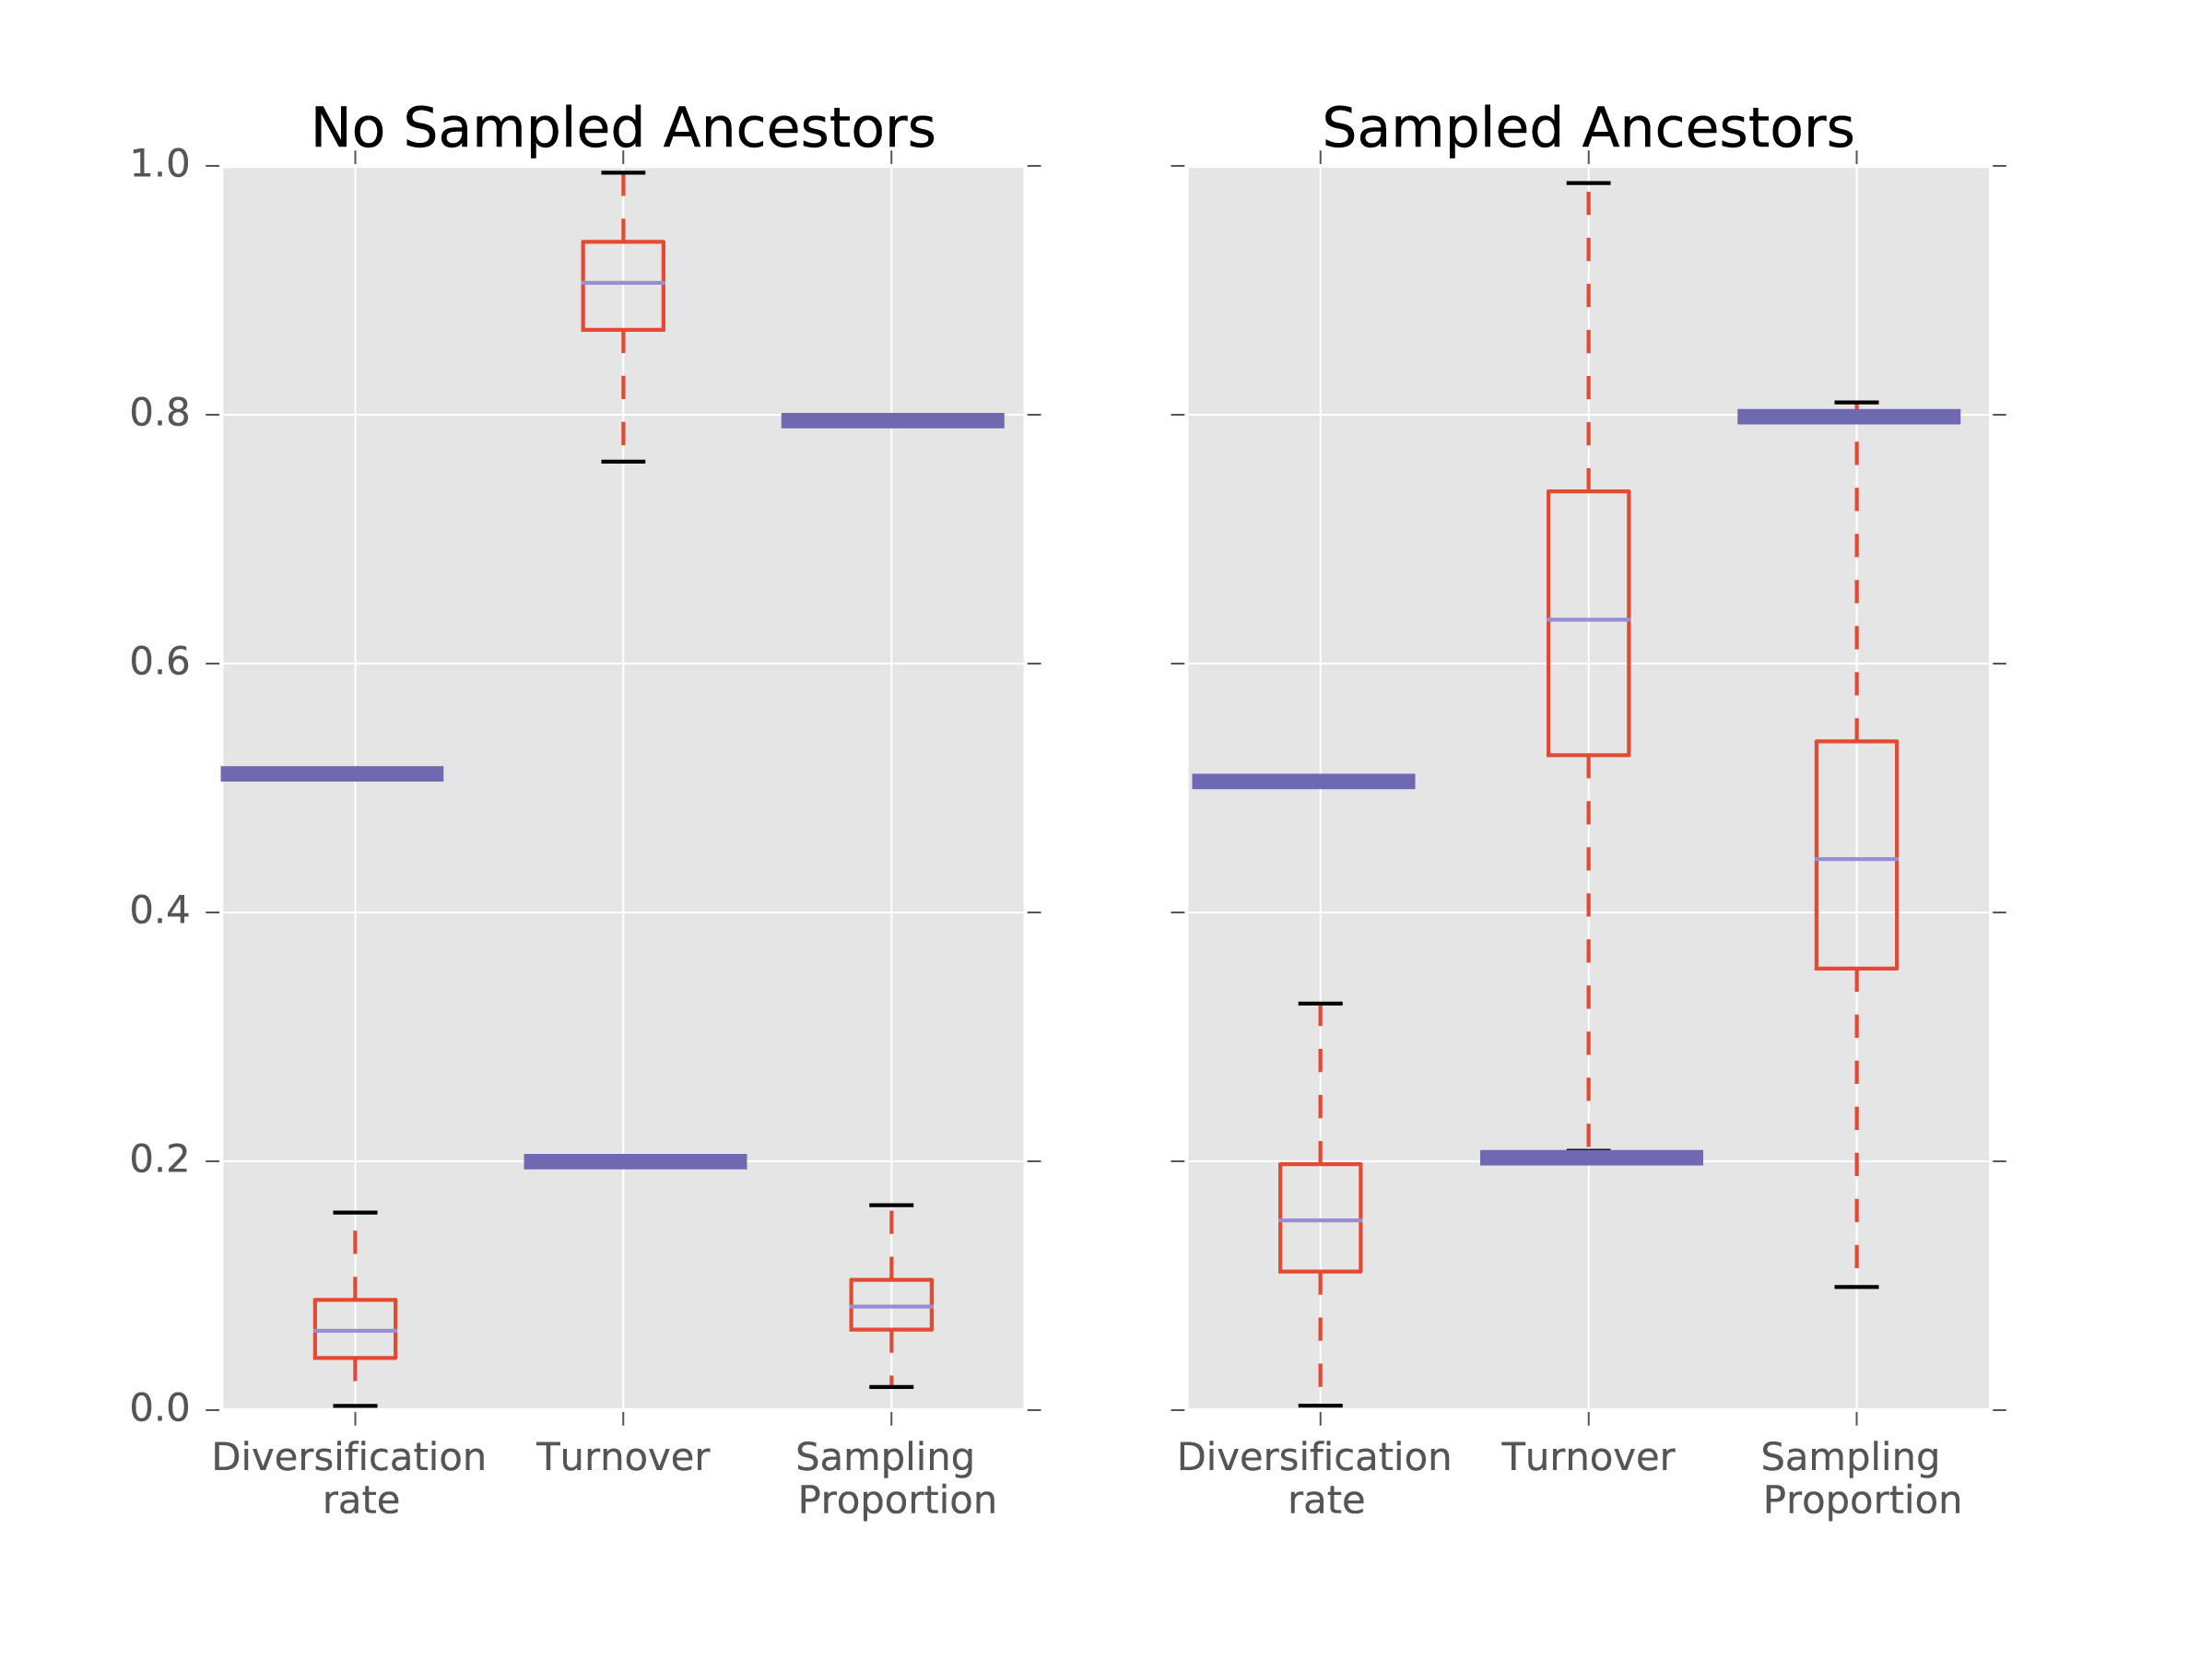
\includegraphics[scale=0.4]{images/LowTurnHighSamplog}
\end{figure}
\end{center}
\end{frame}


\begin{frame}
\frametitle{Results -  Simulations}
\begin{center}
\begin{figure}
High turnover, high sampling  \\
82\% of fossils are sampled ancestors \\
\mathlarger{\mathlarger{\mathlarger{\boldsymbol{\lambda}}}} \mu \psi   \rho \\
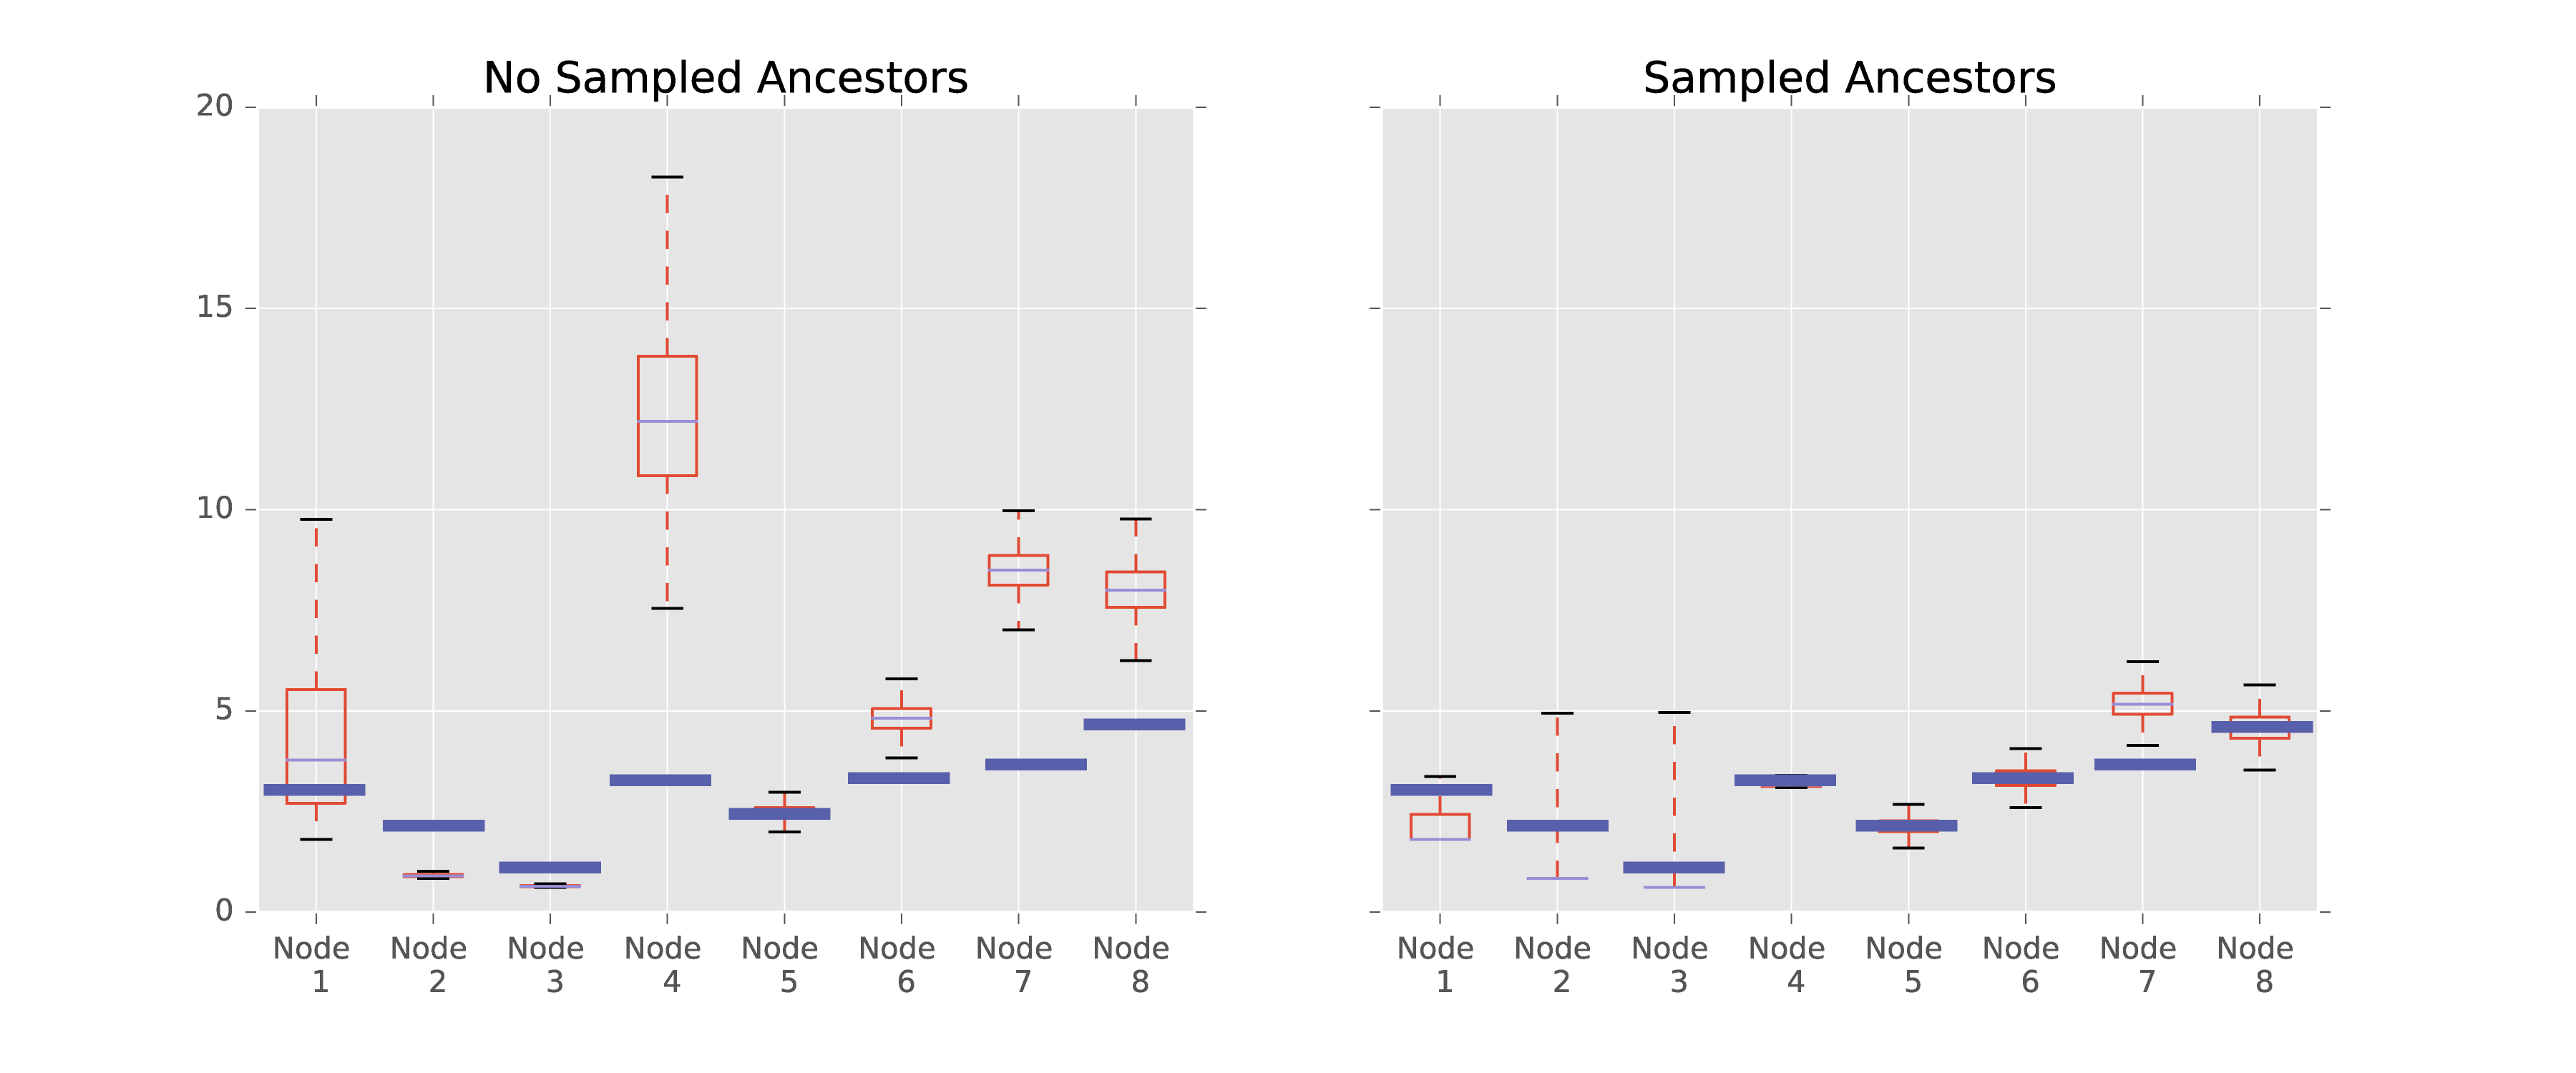
\includegraphics[scale=0.4]{images/HighTurnHighSampnodes}
\end{figure}
\end{center}
\end{frame}


\begin{frame}
\frametitle{Results - Empirical}
\includegraphics[scale=.3]{images/Combined}
\end{frame}

\begin{frame}
\frametitle{Results - Empirical}
\includegraphics[scale=.5]{images/SACount}
\end{frame}


\begin{frame}
\frametitle{Conclusions}
Modeling datasets with sampled ancestors using a non-sampled ancestor model may result in older node age estimates
\end{frame}

\begin{frame}
\frametitle{Conclusions}
Modeling datasets with sampled ancestors using a non-sampled ancestor model may result in older node ages estimates
\begin{itemize}
\item Model parameter estimates (\(\lambda, \mu \) ) are also affected by model misspecification
\end{itemize}
\end{frame}

\begin{frame}
\frametitle{Conclusions}
Modeling datasets with sampled ancestors using a non-sampled ancestor model may result in older node ages estimates
\begin{itemize}
\item Model parameter estimates (\(\lambda, \mu \) ) are also affected by model misspecification
\item The effect increases with the number of sampled ancestors
\end{itemize}
\end{frame}

\begin{frame}
\frametitle{Conclusions}
Modeling datasets with sampled ancestors using a non-sampled ancestor model may result in older node ages estimates
\begin{itemize}
\item Model parameter estimates (\(\lambda, \mu \) ) are also affected by model misspecification
\item The effect increases with the number of sampled ancestors
\item The presence of sampled ancestors becomes more likely as turnover increases
\end{itemize}
\end{frame}

\begin{frame}
\frametitle{Thank You!}

\end{itemize}
\end{frame}


\end{document}